\documentclass[12pt,letterpaper]{article}
\usepackage{graphicx,textcomp}
\usepackage{natbib}
\usepackage{setspace}
\usepackage{fullpage}
\usepackage{color}
\usepackage[reqno]{amsmath}
\usepackage{amsthm}
\usepackage{fancyvrb}
\usepackage{amssymb,enumerate}
\usepackage[all]{xy}
\usepackage{endnotes}
\usepackage{lscape}
\newtheorem{com}{Comment}
\usepackage{float}
\usepackage{hyperref}
\newtheorem{lem} {Lemma}
\newtheorem{prop}{Proposition}
\newtheorem{thm}{Theorem}
\newtheorem{defn}{Definition}
\newtheorem{cor}{Corollary}
\newtheorem{obs}{Observation}
\usepackage[compact]{titlesec}
\usepackage{dcolumn}
\usepackage{tikz}
\usetikzlibrary{arrows}
\usepackage{multirow}
\usepackage{xcolor}
\newcolumntype{.}{D{.}{.}{-1}}
\newcolumntype{d}[1]{D{.}{.}{#1}}
\definecolor{light-gray}{gray}{0.65}
\usepackage{url}
\usepackage{listings}
\usepackage{color}

\definecolor{codegreen}{rgb}{0,0.6,0}
\definecolor{codegray}{rgb}{0.5,0.5,0.5}
\definecolor{codepurple}{rgb}{0.58,0,0.82}
\definecolor{backcolour}{rgb}{0.95,0.95,0.92}

\lstdefinestyle{mystyle}{
	backgroundcolor=\color{backcolour},   
	commentstyle=\color{codegreen},
	keywordstyle=\color{magenta},
	numberstyle=\tiny\color{codegray},
	stringstyle=\color{codepurple},
	basicstyle=\footnotesize,
	breakatwhitespace=false,         
	breaklines=true,                 
	captionpos=b,                    
	keepspaces=true,                 
	numbers=left,                    
	numbersep=5pt,                  
	showspaces=false,                
	showstringspaces=false,
	showtabs=false,                  
	tabsize=2
}
\lstset{style=mystyle}
\newcommand{\Sref}[1]{Section~\ref{#1}}
\newtheorem{hyp}{Hypothesis}

\title{Problem Set 4}
\date{Due: April 12, 2024}
\author{Applied Stats II}


\begin{document}
	\maketitle
	\section*{Instructions}
	\begin{itemize}
	\item Please show your work! You may lose points by simply writing in the answer. If the problem requires you to execute commands in \texttt{R}, please include the code you used to get your answers. Please also include the \texttt{.R} file that contains your code. If you are not sure if work needs to be shown for a particular problem, please ask.
	\item Your homework should be submitted electronically on GitHub in \texttt{.pdf} form.
	\item This problem set is due before 23:59 on Friday April 12, 2024. No late assignments will be accepted.

	\end{itemize}

	\vspace{.25cm}
\section*{Question 1}
\vspace{.25cm}
\noindent We're interested in modeling the historical causes of child mortality. We have data from 26855 children born in Skellefteå, Sweden from 1850 to 1884. Using the "child" dataset in the \texttt{eha} library, fit a Cox Proportional Hazard model using mother's age and infant's gender as covariates. Present and interpret the output.

\vspace{.5cm}
\lstinputlisting [language=R, firstline=1, lastline=42]{PS4.R} 
\begin{figure}[h!] % Use [h!] to try and place the image 'here'
	\centering % Centers the image
	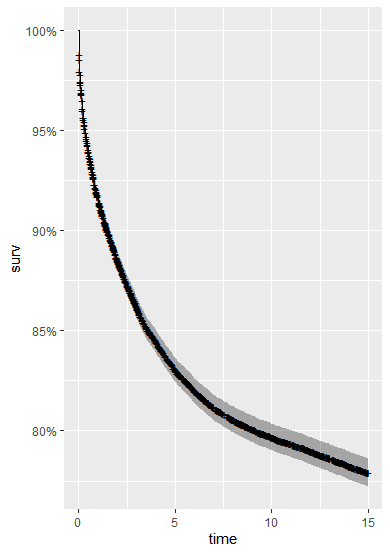
\includegraphics[width=0.7\textwidth]{Rplot.png} % Adjust width as needed
	\caption{Survival Curve of Cox Model} 
	\label{fig:myplot} % A label for referencing in your text 
\end{figure}
\end{document}
